% MIT License

% Copyright (c) 2020 Simon Crase

% Permission is hereby granted, free of charge, to any person obtaining a copy
% of this software and associated documentation files (the "Software"), to deal
% in the Software without restriction, including without limitation the rights
% to use, copy, modify, merge, publish, distribute, sublicense, and/or sell
% copies of the Software, and to permit persons to whom the Software is
% furnished to do so, subject to the following conditions:

% The above copyright notice and this permission notice shall be included in all
% copies or substantial portions of the Software.

% THE SOFTWARE IS PROVIDED "AS IS", WITHOUT WARRANTY OF ANY KIND, EXPRESS OR
% IMPLIED, INCLUDING BUT NOT LIMITED TO THE WARRANTIES OF MERCHANTABILITY,
% FITNESS FOR A PARTICULAR PURPOSE AND NONINFRINGEMENT. IN NO EVENT SHALL THE
% AUTHORS OR COPYRIGHT HOLDERS BE LIABLE FOR ANY CLAIM, DAMAGES OR OTHER
% LIABILITY, WHETHER IN AN ACTION OF CONTRACT, TORT OR OTHERWISE, ARISING FROM,
% OUT OF OR IN CONNECTION WITH THE SOFTWARE OR THE USE OR OTHER DEALINGS IN THE
% SOFTWARE.

\documentclass[]{article}
\usepackage{caption,subcaption,graphicx,float,url,amsmath,amssymb,tocloft,cancel,amsthm,thmtools}
\usepackage[hidelinks]{hyperref}
\usepackage[toc,acronym,nonumberlist]{glossaries}
\usepackage{titling}
\setacronymstyle{long-short}
\usepackage{glossaries-extra}
\usepackage[]{algorithm2e}

\graphicspath{{figs/}} 
\setlength{\cftsubsecindent}{0em}
\setlength{\cftsecnumwidth}{3em}
\setlength{\cftsubsecnumwidth}{3em}
% I snarfed the next line from Stack exchange
% https://tex.stackexchange.com/questions
%    /42726/align-but-show-one-equation-number-at-the-end
% It allows me to suppress equation numbers with align*,
% then selectively add equation numbers
% for lines that I want to reference slsewhere
\newcommand\numberthis{\addtocounter{equation}{1}\tag{\theequation}}
\newtheorem{thm}{Theorem}
\newtheorem{conj}{Conjecture}

%opening
\title{
	Notes from \\
	Computation in Complex Systems
}
\author{Simon Crase (compiler)\\simon@greenweaves.nz}

\makeglossaries

\renewcommand{\glstextformat}[1]{\textbf{\em #1}}

\begin{document}

\maketitle

\begin{abstract}
   These are my notes from Computation in Complex Systems\cite{sfi2020computation}\\
   The content and images contained herein are the intellectual property of the Santa Fe Institute, with the exception of any errors in transcription, which are my own.
   These notes are distributed in the hope that they will be useful,
   but without any warranty, and without even the implied warranty of
   merchantability or fitness for a particular purpose. All feedback is welcome,
   but I don't necessarily undertake to do anything with it.\\
   \LaTeX source for the notes can be found at\\
   \url{https://github.com/weka511/complexity/tree/master/computations}.
\end{abstract}

\setcounter{tocdepth}{2}
\tableofcontents

\listoffigures
\listoftheorems[ignoreall,onlynamed]

\newglossaryentry{gls:3:SAT}{
	name={3-SAT},
	description={Given a set of \glspl{gls:clause} with 3 variables (or negated variables) each, e.g. $(x_1 \lor \bar{x_2} \lor x_3) \land (x_2 \lor x_{17} \lor \bar{x_{23}}) \land...$ is there a set $\{x_i\}$ such that all clauses are satisfied?}}

\newglossaryentry{gls:clause}{
	name={clause},
	description={In logic, a clause is an expression formed from a finite collection of literals (atoms or their negations) }}

\newglossaryentry{gls:clustering}{
	name={Clustering Transition},
	description={This means that here the organization of the space of the exponentially many degenerate solutions changes from one big cluster ($\alpha<\alpha_C$) of solutions which are connected in assignment space to a solution space ($\alpha>\alpha_C$) which is fragmented into many non-connected smaller clusters, one says replica symmetry is broken above this threshold\cite{schawe2019phase}}}

\newglossaryentry{gls:condensation}{
	name={Condensation Transition},
	description={Below this thrshold, the measure is evenly split among an exponential number of clusters. Above itthe measure is carried by a subexponential number of clusters.\cite{krzakala2007gibbs}}}


\newglossaryentry{gls:eulerian:path}{
	name={Eulerian path},
	description={In graph theory, an Eulerian path is a path in a finite graph that visits every edge exactly once (allowing for revisiting vertices) }}

\newglossaryentry{gls:eulerian:cycle}{
	name={Eulerian cycle},
	description={Similarly, an Eulerian circuit or Eulerian cycle is an \gls{gls:eulerian:path} that starts and ends on the same vertex. }}

\newglossaryentry{gls:freezing}{
	name={Freezing Transition},
	description={The smallest density of constraints $\alpha$ such that all solutions belong to frozen clusters\cite{ardelius2008exhaustive}}}

\newglossaryentry{gls:Hamiltonian:cycle}{
	name={Hamiltonian cycle},
	description={If a \gls{gls:Hamiltonian:path} exists whose endpoints are adjacent, then the resulting graph cycle is called a Hamiltonian cycle (or Hamiltonian cycle) }}

\newglossaryentry{gls:Hamiltonian:path}{
	name={Hamiltonian path},
	description={A Hamiltonian path, also called a Hamilton path, is a graph path between two vertices of a graph that visits each vertex exactly once }}

\newglossaryentry{gls:k:SAT}{
	name={k-SAT},
	description={Given a set of \glspl{gls:clause} with $k$ variables (or negated variables) each, is there a set $\{x_i\}$ such that all clauses are satisfied?}}

\newglossaryentry {gls:NAESAT} {
	name={NAESAT},
	description={An NAESAT clause is one of the form: $$
		(x_1 \lor x_2 \lor x_3) \land (\bar{x_1} \lor \bar{x_2} \lor \bar{x_3})
		$$}}
	
\newglossaryentry{gls:NonDP}{
	name={Non-deterministic Polynomial Time},
	description={we can \emph{check} a solution efficiently}}

\newglossaryentry{gls:NP:complete}{
	name={NP-Complete},
	description={It turns out that there are problems $B$ in \gls{gls:NP} such that any other problem $A$  in \gls{gls:NP} can be \gls{gls:reduced} to $B$: $A \le B \forall A \in NP$. Such a $B$ is said to be NP-Complete}}

\newglossaryentry{gls:O}{
	name={O},
	description={$f(n)=O(n^3)$ means: when $n$ is large $f(n)$ scales as $n^3$ or less. Formally:
	\begin{align*}
		f(n) =& O(g(n))\\
		\equiv&	\;\; \exists C, n_0 \text{ such that}\\
		 \forall n>n_0, f(n) \le& Cg(n)
	\end{align*}}}

\newglossaryentry{gls:o}{
	name={o},
	description={$f$ grows more slowly than $g$: $f/g \rightarrow 0 \text{ as } n\rightarrow \infty$}}

\newglossaryentry{gls:Omega}{
	name={$\Omega$},
	description={$f$ grows at least as fast as $g$: $g=O(f)$ : $f/g \cancel{\rightarrow} 0 \text{ as } n\rightarrow \infty$}}

\newglossaryentry{gls:pr}{
	name={primitive recursive function},description={Primitive recursive functions are those defined by composition and primitive recursion.}}

\newglossaryentry{gls:Polynomial}{
	name={Polynomial Time},
	description={we can find a solution efficiently}}

\newglossaryentry{gls:PSPACE}{
	name={PSPACE},
	description={problems we can solve with a polynomial amout of memory, even if they take an infinire amount of time.}}

\newglossaryentry{gls:reduced}{
	name={reduced},
	description={$A$ can be \emph{reduced} to $B$, or $A \le B$, if there is a polynomial algorithm that translated instances of $A$ to instances of $B$, so the yes/no answer stays the same. }}

\newglossaryentry{gls:Theta}{
	name={$\Theta$},
	description={$f$ and $g$ grow the same way: $g=O(f)$ and $f=O(g)$ or $f/g \rightarrow C>0\text{ as } n\rightarrow \infty$}}

\newglossaryentry{gls:xorsat}{
	name={XORSAT},
	description={Similar to SAT, except we demand that an odd number of terms in each clause be true}}

\newacronym[see={[Glossary:]{gls:Polynomial}}]{gls:P}{P}{Polynomial\glsadd{gls:Polynomial}}

\newacronym[see={[Glossary:]{gls:NonDP}}]{gls:NP}{NP}{Non-deterministic Polynomial\glsadd{gls:NonDP}}

\section{Easy \& Hard}


For theorists, polynomial vs. exponential is the mark of insight: we have found some structure in the problem that we can use.

\subsection{Two Kinds of Paths}

\begin{figure}[H]
	\caption{Eulerian paths}
	\begin{subfigure}[t]{0.54\textwidth}
		\caption{The 7 bridges of K\"onigsberg: can we cross each bridge only once? One strategy is brute force search.}
		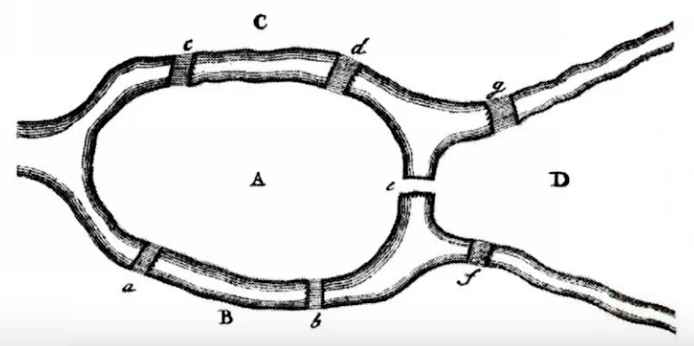
\includegraphics[width=\textwidth]{euler}
	\end{subfigure}
	\begin{subfigure}[t]{0.54\textwidth}
		\caption{Euler: if a tour exists, at most 2 noded can have an odd number of bridges, so no tour is possible. Much faster.}
		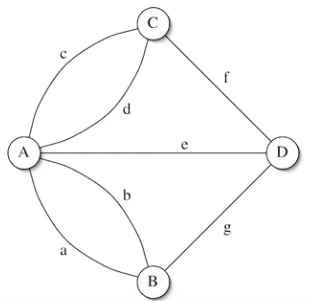
\includegraphics[width=\textwidth]{euler2}
	\end{subfigure}
\end{figure}

\begin{figure}[H]
	\begin{center}
		\caption{Hamiltonian Path: visit each node once}
		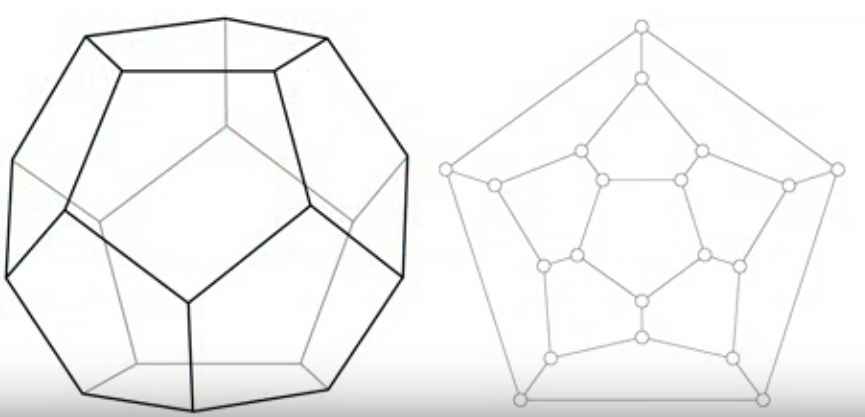
\includegraphics[width=\textwidth]{Hamiltonian}
	\end{center}
\end{figure}

\subsection{Polynomials vs. Exponentials}

Polynomials don't grow too fast Figure \ref{fig:polynomial} compared to exponential \ref{fig:exponential}.
\begin{figure}[H]
	\caption{Polynomials don't grow too fast}\label{fig:polynomial} 
	\begin{subfigure}[t]{0.3\textwidth}
		\caption{}
		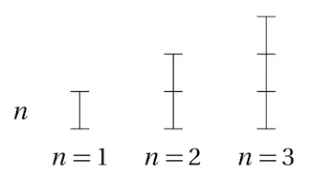
\includegraphics[width=\textwidth]{n1}
	\end{subfigure}
	\begin{subfigure}[t]{0.3\textwidth}
		\caption{}
		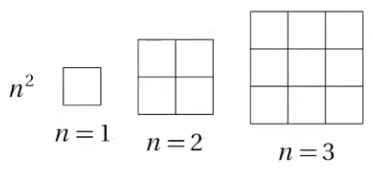
\includegraphics[width=\textwidth]{n2}
	\end{subfigure}
	\begin{subfigure}[t]{0.3\textwidth}
		\caption{}
		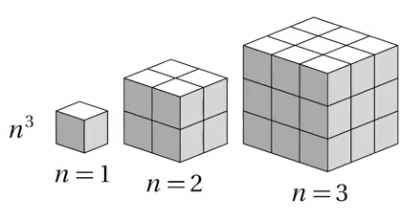
\includegraphics[width=\textwidth]{n3}
	\end{subfigure}
\end{figure}

\begin{figure}[H]
	\begin{center}
		\caption{Exponential Growth: this is what we don't want.}\label{fig:exponential}
		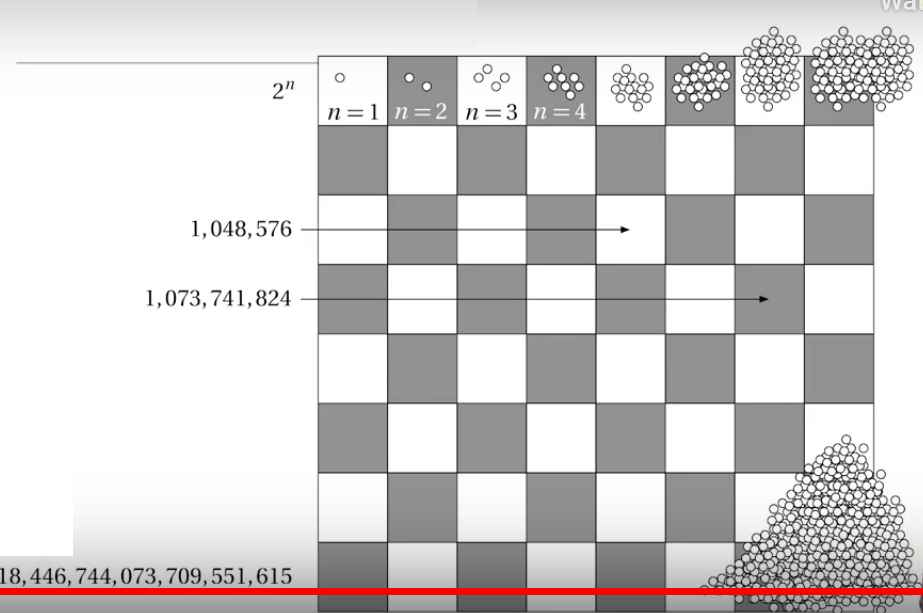
\includegraphics[width=0.8\textwidth]{exponential}
	\end{center}
\end{figure}
\subsection{Divide and Conquer}

\begin{figure}[H]
	\begin{center}
		\caption[Towers of Hanoi]{Towers of Hanoi. Figure \ref{fig:towers-hanoi-rb} shows how to break the problem--Figure \ref{fig:towers-hanoi}--down recursively.}\label{fig:toh}
		\begin{subfigure}[t]{0.35\textwidth}
			\caption{The problem}\label{fig:towers-hanoi}
			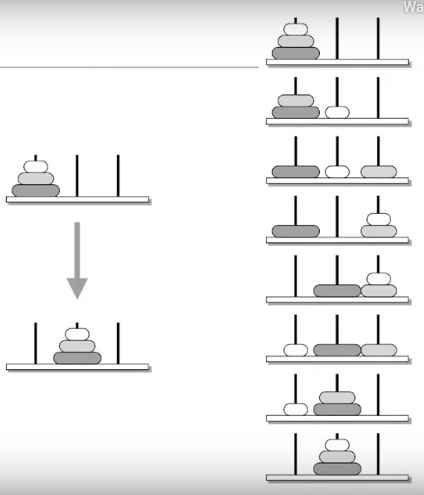
\includegraphics[width=\textwidth]{towers-hanoi}
		\end{subfigure}
		\begin{subfigure}[t]{0.6\textwidth}
			\caption{Recursive breakdown}\label{fig:towers-hanoi-rb}
			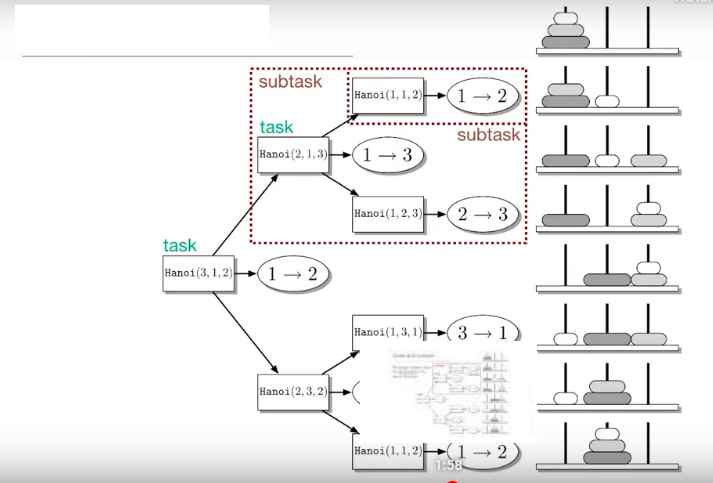
\includegraphics[width=\textwidth]{towers-hanoi-breakdown}
		\end{subfigure}
	\end{center}
\end{figure}

How many moves are needed for $n$ disks?
\begin{align*}
	f(0) =& 0 \\
	f(n) =& 2f(n-1) + 1\\
	=& 2^n -1
\end{align*}

\subsection{Big O and All that}

In computer science, a real problem is an infinite family of examples or instances. How much of some resource--time, memory, etc--do we need as a function of $n$?

\begin{itemize}
	\item \gls{gls:O} \glsdesc{gls:O}
	\item \gls{gls:Omega} \glsdesc{gls:Omega}
	\item \gls{gls:o} \glsdesc{gls:o}
	\item \gls{gls:Theta} \glsdesc{gls:Theta}
\end{itemize}

\subsection{When the details don't matter}

Polynomials vs. Exponentials.

\begin{itemize}
	\item relates to whether we can exploit some feature or are just searching;
	\item releases us from many of the details.
	\begin{itemize}
		\item The size of an instance is the number of bits to describe it, e.g. the number of bits in an email.
		\item For polynomial versus exponential, the description format doesn't matter: e.g. we can describe a network as an $n^2$ adjacency matrix, or as notes with links $n\log(n)$, but this just changes one polynomial to another.
		\item Data storage formats don't turn polynomial into exponential, e.g. linear list ($n$) versus tree ($\log(n)$) 
		\item Neither does technology--e.g. RAM vs. magnetic tape--Figure \ref{fig:imb729mtu}--$T$ vs. $T^2$.
	\end{itemize}
\end{itemize}

\begin{figure}[H]
	\begin{center}
		\caption{IBM 729 Magnetic Tape Unit}\label{fig:imb729mtu}
		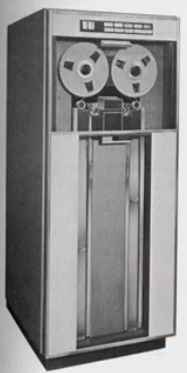
\includegraphics[width=0.6\textwidth]{imb729mtu}
	\end{center}
\end{figure}

References: \cite[Chapters 1,2,4]{moore2011nature}

\section{Algorithms and Landscapes}


\subsection{Divide and Conquer Redux}

How long does it take to sort a list of $n$ numbers? We could think of this as a search through $n!$ possibilities.

\begin{figure}[H]
	\caption{Mergesort: recursively split list in half, sort the halves, and merge.}\label{fig:mergesort}
	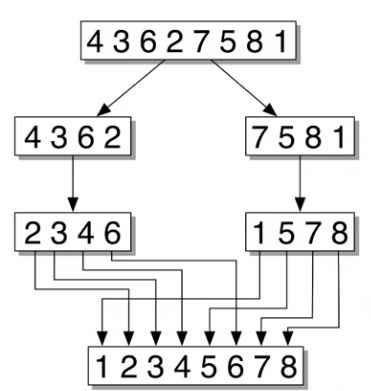
\includegraphics[width=0.8\textwidth]{mergesort}
\end{figure}

Estimate the time to sort n items by $T(n)$, the number of comparisons.
\begin{align*}
T(1) =& 0 \text{. already sorted}\\
T(n) =&\underbrace{ 2T(\frac{n}{2})}_\text{Two sorts of hald length} + \underbrace{n}_\text{Merge} \text{, hence}\\
=& n \log_2(n)
\end{align*}

\begin{table}[H]
	\begin{center}
		\caption{Number of comparisons for mergesort}
		\begin{tabular}{|r|r|} \hline
			$n$&$T(n)$  \\ \hline
			1& 0\\ \hline
			2&2 \\ \hline
			4&8 \\ \hline
			8& 24\\ \hline
			16& 64\\ \hline
			32& 160\\ \hline
		\end{tabular}
	\end{center}
\end{table}


\subsection{Dynamic Programming}

\begin{align*}
	d(s,t)=& \min(d(s^\prime,t)+1, d(s,t^\prime)+1,d(s^\prime,t^\prime) + \delta(s_1,t_1)) \text{ , where}\\
	d(s,t)=& \text{ number of changes to convert $s$ to $d$}\\
	s^\prime=& \text{ string $s$ with 1st character, $s_1$ removed}\\
	t^\prime=& \text{ string $t$ with 1st character, $t_1$ removed}
\end{align*}

There are only $n^2$ sub-problems: polynomial time.

\subsection{Greedy Algorithms}

\begin{figure}[H]
	\caption{Minimum Spanning Tree}
	\begin{subfigure}[t]{0.45\textwidth}
		\caption{e.g. power lines}
		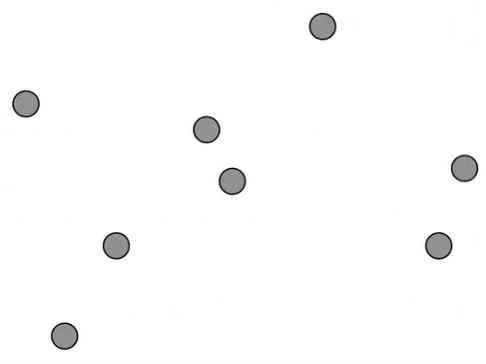
\includegraphics[width=\textwidth]{mst1}
	\end{subfigure}
	\;\;\;
	\begin{subfigure}[t]{0.45\textwidth}
		\caption{Start by adding the shortest edge}
		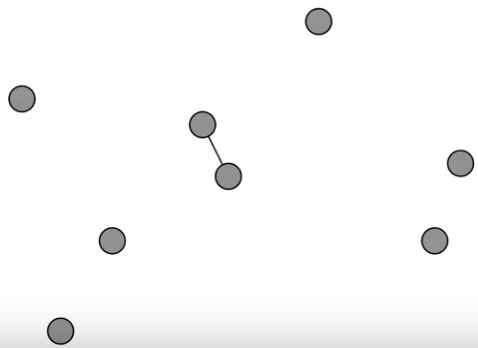
\includegraphics[width=\textwidth]{mst2}
	\end{subfigure}
	\begin{subfigure}[b]{0.45\textwidth}
		\caption{At each step, add the shortest edge that doesn't complete a cycle}
		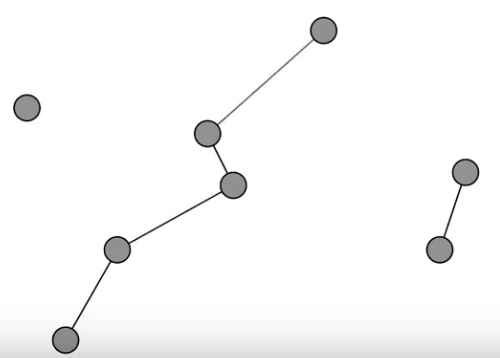
\includegraphics[width=\textwidth]{mst3}
	\end{subfigure}
	\;\;\;
	\begin{subfigure}[b]{0.45\textwidth}
		\caption{The complete tree}\label{fig:mst4}
		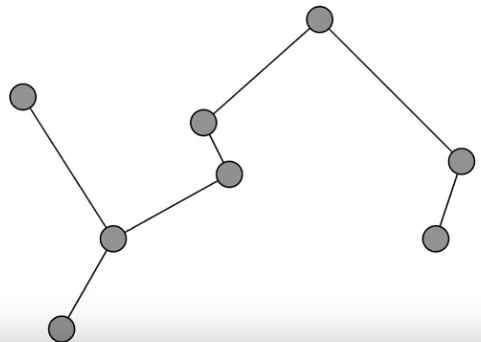
\includegraphics[width=\textwidth]{mst4}
	\end{subfigure}
\end{figure}

Clearly Figure \ref{fig:mst4} is \emph{a} spanning tree, but how do we know it is minimal?

\begin{figure}[H]
	\caption{How do we know Figure \ref{fig:mst4} is minimal?}
	\begin{subfigure}[b]{0.30\textwidth}
		\caption{Let $e$ be the shortest edge that doesn't complete a cycle, and suppose that the minimum spanning tree $T$ doesn't contain $e$}
		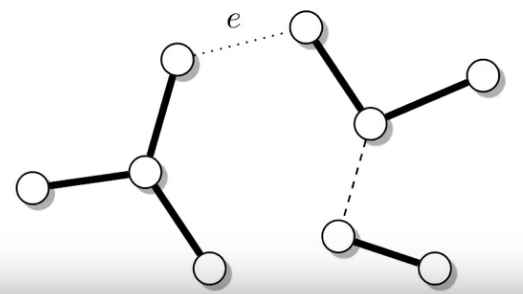
\includegraphics[width=\textwidth]{mst5}
	\end{subfigure}
	\;\;\;
	\begin{subfigure}[b]{0.30\textwidth}
		\caption{Then there must be some other path from one end of $e$ to another that goes through a longer edge $e^\prime$.}
		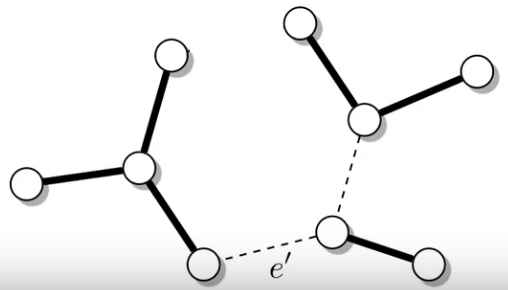
\includegraphics[width=\textwidth]{mst6}
	\end{subfigure}
	\;\;\;
	\begin{subfigure}[b]{0.30\textwidth}
		\caption{But then we could reduce the total length by deleting $e^\prime$ and adding $e$--a contradiction.}
		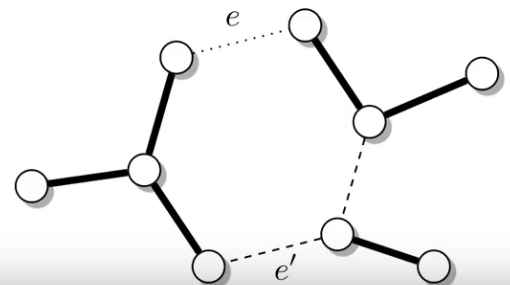
\includegraphics[width=\textwidth]{mst7}
	\end{subfigure}
\end{figure}

Greed isn't always good, or even very often good--Figures \ref{fig:greedy:tsp} and \ref{fig:lessgreedy:tsp}.
\begin{figure}[H]
	\caption{Travelling Salesman Problem}
	\begin{subfigure}[t]{0.45\textwidth}
		\caption{Greedy solution to Travelling Salesman Problem}\label{fig:greedy:tsp}
		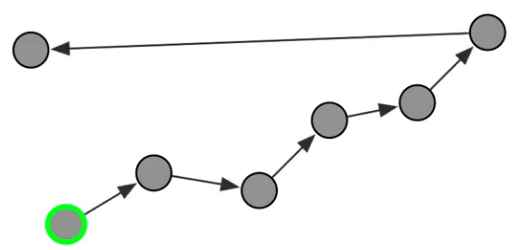
\includegraphics[width=\textwidth]{tsp1}
	\end{subfigure}
	\;\;\;
	\begin{subfigure}[t]{0.45\textwidth}
		\caption{A less Greedy solution is somewhat better}\label{fig:lessgreedy:tsp}
		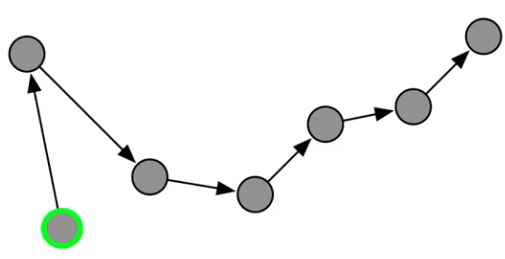
\includegraphics[width=\textwidth]{tsp2}
	\end{subfigure}
\end{figure}

\subsection{Landscapes}

\subsubsection{Greedy Algorithms and the Fitness Landscape}

\begin{figure}[H]
	\caption{Greedy Algorithms and the Fitness Landscape}
	\begin{subfigure}[t]{0.4\textwidth}
		\caption{A greedy algorithm works well if the Fitness Landscape looks like Fuji-San}
		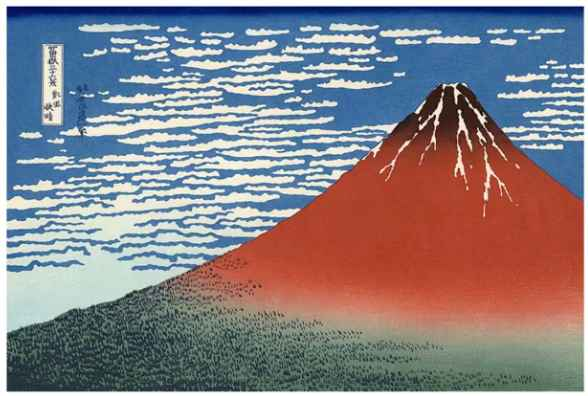
\includegraphics[width=\textwidth]{fujisan}
	\end{subfigure}
	\;\;\;
	\begin{subfigure}[t]{0.55\textwidth}
		\caption{A Greedy solution doesn't work well if there are many local optima where we can get stuck: it cannot cross a valley to get to a higher peak.}
		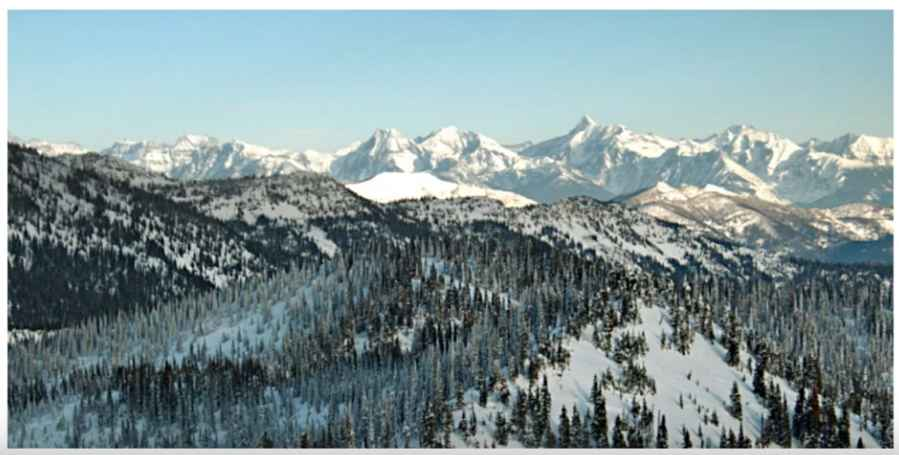
\includegraphics[width=\textwidth]{rockies}
	\end{subfigure}
\end{figure}

\subsubsection{Reorganizing the Landscape}

What defines the neighbourhood? When is one solution close to another?

\begin{figure}[H]
	\caption[Maxflow: determine the maximum flow from $s$ to $t$]{Maxflow: take a network such as \ref{fig:maxflow1} and determine the maximum flow from $s$ to $t$. We can see that we can eliminate local optima by allowing a new kind of move. By expanding our idea of what kins of solutions are neighbours we reorganize the landscape!}
	\begin{subfigure}[t]{0.4\textwidth}
		\caption{Each edge has a capacity}\label{fig:maxflow1}
		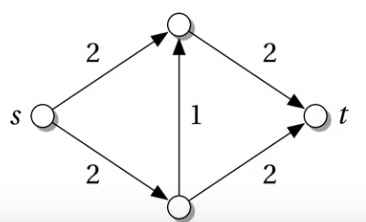
\includegraphics[width=\textwidth]{maxflow1}
	\end{subfigure}
	\;\;\;
	\begin{subfigure}[t]{0.55\textwidth}
		\caption{Greedy: push more flow along a channel with excess capacity. But we can get stuck at a local optimum. Here we have three units flowing--we are at a local optimum.}\label{fig:maxflow2}
		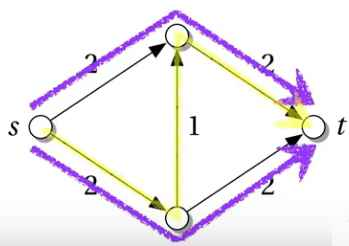
\includegraphics[width=\textwidth]{maxflow2}
	\end{subfigure}
	\;\;\;
	\begin{subfigure}[t]{0.45\textwidth}
		\caption{We should have done this instead}\label{fig:maxflow3}
		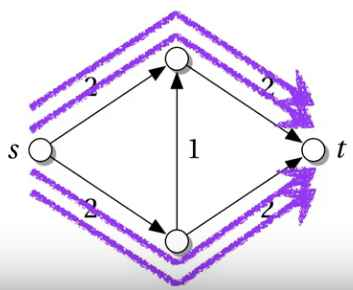
\includegraphics[width=\textwidth]{maxflow3}
	\end{subfigure}
	\;\;\;
	\begin{subfigure}[t]{0.45\textwidth}
		\caption{Allow reverse edges to cancel previous flow: now if we add to Figure \ref{fig:maxflow2} we get the optimum--Figure \ref{fig:maxflow3}. If we allow this type of move we can never get stuck: there are no local optima.}
		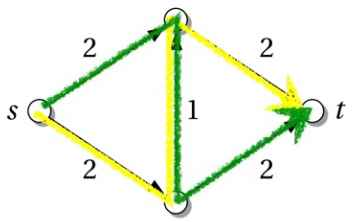
\includegraphics[width=\textwidth]{maxflow4}
	\end{subfigure}
\end{figure}

This won't always work. Some problems are inherently bumpy.

\subsection{Reductions and Translations}

\begin{figure}[H]
	\caption[Reducing one problem into another]{Reducing one problem into another. We want a perfect bipartite matching, where everyone has a partner. This is a subset of the edges of this graph, so everyone on one side is connected to exactly one person on the other. There are $n!$ possible matchings.}
	\begin{subfigure}[t]{0.3\textwidth}
		\caption{Bipartite Graph. }
		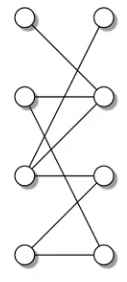
\includegraphics[width=\textwidth]{bpg1}
	\end{subfigure}
	\;\;\;
	\begin{subfigure}[t]{0.65\textwidth}
		\caption{We can transform the problem to max flow. Each compatible couple becomes an edge with flow 1.}
		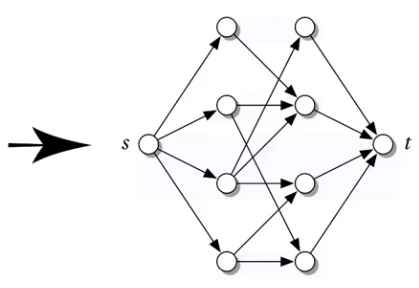
\includegraphics[width=\textwidth]{bpg2}
	\end{subfigure}
\end{figure}

\begin{thm}[Maxflow]
	If all the flows have integral capacities, the solution is also integral.
\end{thm}

In terms of complexity, Bipartite Matching $\le$ Max Flow.


\begin{figure}[H]
	\caption{Shortest Path}
	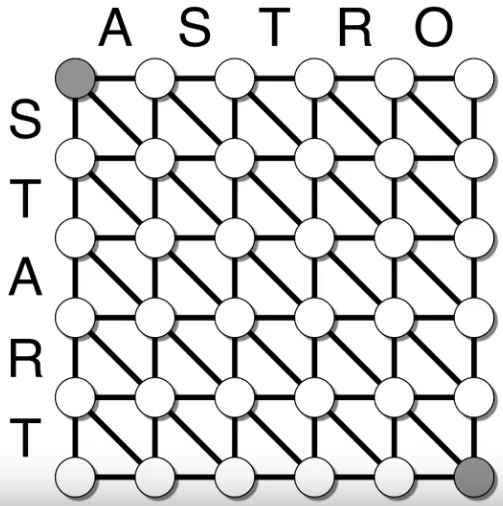
\includegraphics[width=0.8\textwidth]{sp1}
\end{figure}

\subsection{Lessons So Far}

We have just a few techniques that are guaranteed to be efficient:
\begin{itemize}
	\item divide and conquer;
	\item dynamic programming;
	\item greedy (local search);
	\item linear programming, convex programming and duality (max-flow and min-cut).
\end{itemize}
These are essentially all we know about: is that all there is?

\subsection{The Best of All Possible Algorithms}

How do we know whether an algorithm is optimal? How long does it take to multiply two $n$ digit numbers? The algorithm we learned in primary school takes time $\propto n^2$. 

\begin{figure}[H]
	\begin{center}
		\caption{What if we try divide and conquer?}
		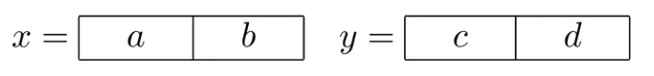
\includegraphics[width=0.6\textwidth]{dc-mult}
	\end{center}
\end{figure}

\begin{align*}
	x=& 10^\frac{n}{2}a+b\\
	y =& 10^\frac{n}{2}c+d\\
	xy=& 10^n a c + 10^\frac{n}{2}(ad+bc) + bd \numberthis \label{eq:xy}
\end{align*}
Multiplication is typically slower than add and shifting. We replace one multiplication of $n$ digit numbers with 4 multiplications of $\frac{n}{2}$ numbers: $T(n) \approx 4T(\frac{n}{2})$. But maybe we can be a bit more clever.

\begin{align*}
	(a+b)(c+d) -ac -bd =& ad+bc 
\end{align*}

We can evaluate (\ref{eq:xy}) with only 3 multiplications, and the running time is now governed by $T(n) \approx 3T(\frac{n}{2})$.

We will solve the equation for T.
\begin{align*}
	T(n) =&3T(\frac{n}{2}) \text{, we want a solution of the form}\\
	T(n) \propto& n^\alpha \text{, whence}\\
	\cancel{n}^\alpha =& 3\big(\frac{\cancel{n}}{2}\big)^\alpha\\
	2^\alpha =& 3\\
	\alpha \log(2) =& \log(3)\\
	\alpha =& \frac{\log(3)}{\log(2)}\\
	\approxeq& 1.585\\
	T(n) \propto n^{1.585} 
\end{align*}
It turns out that we can get $\alpha$ down as close to 1 as we want.

How does mergesort $n \log_2(n)$ compare with best possible algorithm? Figure \ref{fig:dt-sort} illustrates the decision table for searching. There needs to be  $\log_2(n!) \approx n \log_2(n)$ comparisons: merge sort is about as good as it gets.

\begin{figure}[H]
	\begin{center}
		\caption{Decision Table for Sort}\label{fig:dt-sort}
		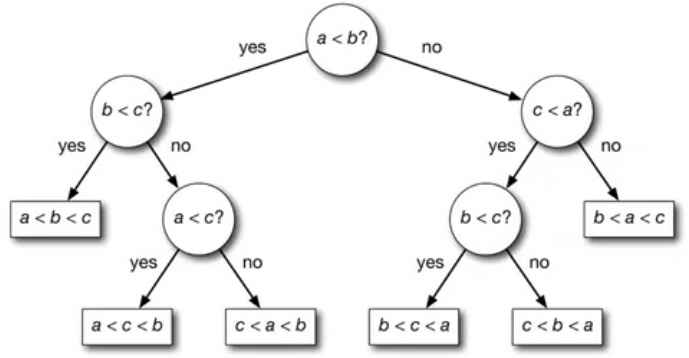
\includegraphics[width=0.6\textwidth]{dt-sort}
	\end{center}
\end{figure}

\subsection{Complexity Wrap-Up}

\begin{itemize}
	\item \emph{Systems} aren't simple or complex; questions about them are.
	\item Intrinsic complexity of a problem: the running time, or memory, or other resource, of the \emph{best possible algorithm}; an objective mathematical fact.
	\item Upper bounds are easy: just give an algorithm.
	\item Lower bounds are hard.
	\item Lower bounds show that one problem is at least as easy (or hard) as another. 
\end{itemize}

References: \cite[Chapter 2]{moore2011nature}

\section{P versus NP}


\subsection{Finding versus Checking}

Some problems can be solved in polynomial time, while other require a brute-force search, which is typically exponential. In the P vs. NP question we deal with ''needles in haystacks'': finding a solution, or telling whether there is one seems hard, by checking a solution is easy.

\begin{figure}[H]
	\begin{center}
		\caption[Hamiltonian path]{\gls{gls:Hamiltonian:path}. We don't know how to solve it in polynomial time, but we can easily check a proposed solution.}\label{fig:PNP1}
		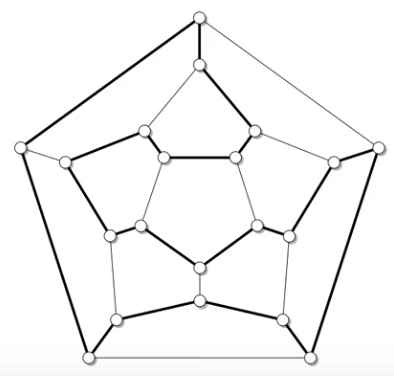
\includegraphics[width=0.8\textwidth]{PNP1}
	\end{center}
\end{figure} 

\begin{itemize}
	\item \gls{gls:P}: \glsdesc{gls:Polynomial}
	\item \gls{gls:NP}: \glsdesc{gls:NonDP}
\end{itemize}

\begin{figure}[H]
	\begin{center}
		\caption[Complexity Classes]{Complexity Classes. We \emph{know} that $P \subseteq NP$, and we \emph{believe} that $P \subset NP$}\label{fig:PNP2}
		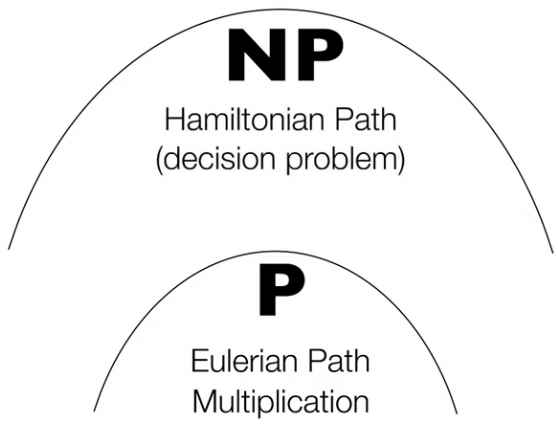
\includegraphics[width=0.8\textwidth]{PNP2}
	\end{center}
\end{figure}

We'll focus on classes of decision problems: not \emph{does this graphs have a \gls{gls:Hamiltonian:path}}, but \emph{can we find a \gls{gls:Hamiltonian:path} for \emph{\gls{gls:Hamiltonian:path}} graph}. We consider \gls{gls:NP:complete} problems.

We say that \glsdesc{gls:reduced} \glsdesc{gls:NP:complete}

But if $A \le B$ and $A$ is hard, them $B$ must be hard too: so $B$ is one of the hardest problems in \gls{gls:NP}. We can therefore focus on one  \gls{gls:NP}: if $B\in NP$ we would know that $P=NP$. Conversely, if $P \ne NP$, $B$ cannot be solved in polynomial time.

Now the Hamiltonian Path problem is NP-Complete: how can such a simple problem represent all \gls{gls:NP} problems?

\subsection{Circuits and Formulae}

Figure \ref{fig:satisfying} illustrates how the question ''is there a \gls{gls:Hamiltonian:path}'' can be transformed to ''are there values for the inputs that make to output \textbf{true}?''
\begin{figure}[H]
	\begin{center}
		\caption{Satisfying a circuit}
		\begin{subfigure}[b]{0.45\textwidth}
			\caption{Satisfying a circuit: any program that tests solutions--e.g. to \gls{gls:Hamiltonian:path}--can be compiled into a Boolean circuit--bits!}\label{fig:satisfying}
			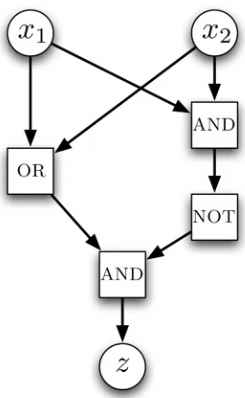
\includegraphics[width=\textwidth]{satisfy}
		\end{subfigure}
		\begin{subfigure}[b]{0.45\textwidth}
			\caption{Add variables representing the truth values of the wires.}\label{fig:add:variables}
			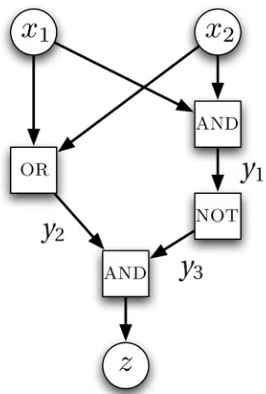
\includegraphics[width=\textwidth]{add-variables}
		\end{subfigure}
	\end{center}
\end{figure}

\begin{align*}
	y = x_1 \land& x_2 \equiv (x_1\lor \bar{y_1}) \land (x_1\lor \bar{y_2}) \land (\bar{x_1} \lor \bar{x_2} \lor y_1)
\end{align*}

We have converted the problem of checking a problem to a program, and than into a problem of checking Boolean expressions. We have therefore reduced out original problem to an instance of \gls{gls:3:SAT}, one of the original 6 \gls{gls:NP:complete} problems.
\glsdesc{gls:3:SAT} \Gls{gls:k:SAT} is ($k$ variables per clause) is \gls{gls:NP:complete} $\forall k \ge 3$.

If \gls{gls:3:SAT} were easy:
\begin{itemize}
	\item we could take any \gls{gls:NP} problem;
	\item write a program that checks a solution;
	\item convert to a circuit;
	\item convert to a 3-SAT formula;
	\item use our efficient 3-SAT solver to solve the original problem;
	\item so if $3-SAT \in P$ then $P=NP$.
	\item If $P\ne NP$, 3-SAT cannot be solved in polynomial time.
\end{itemize}

\begin{thm}[k-SAT $\le$ 3-SAT]
	\gls{gls:k:SAT} $\le$ \gls{gls:3:SAT}
\end{thm}

\begin{proof}
	We can break k-clauses down into 3-clauses, by adding new variables $\{z_i\}$, e.g.:
	\begin{align*}
		(x_1 \lor x_2 \lor x_3 \lor x_4 \lor x_5) =& (x_1 \lor x_2 \lor z_1) \land (\bar{z_1} \lor x_3 \lor z_2) \land (\bar{z_2} \lor x_4 \lor x_5)
	\end{align*}
	so we get 3-SAT clauses. They are good logical building blocks: this isn't true for 2-SAT clauses. A 3-SAT clause has ''chemistry'' and triggers a search. 
\end{proof}

\begin{thm}[2-SAT $\in$ P.]
	2-SAT $\in$ P.
\end{thm}

\begin{proof}
	TBP
\end{proof}

\subsection{More NP-complete Problems}

\begin{itemize}
	\item Polynomial time reduction is transitive: $A \le B \land B \le C\implies A \le C$.
	\item So we can prove a problem is NP-complete by reducing any other problem to it.
	\item e.g. Circuit satisfiability $\le$ 3-SAT.
	\item 3-SAT $\le$ \gls{gls:NAESAT}--\glsdesc{gls:NAESAT}
\end{itemize}

\subsubsection{Not All Equal SAT}

We need to be careful when we reduce to know which direction we are going.
Can we build \gls{gls:3:SAT} out of \gls{gls:NAESAT} building blocks?
\begin{itemize}
	\item \gls{gls:3:SAT} is symmetric: can we build it out of asymmetric parts?
	\item Add a global variable $s$ to break the symmetry.
	\item Consider the NAE-4-SAT clause $(x_1,x_2,x_3,s)$: what if $s$ false? what if it is true?
	\item This translates  \gls{gls:3:SAT} to NAE-4-SAT. Then we can use the same trick we used above for \gls{gls:k:SAT} to reduce  NAE-4-SAT to NAE-3-SAT.
\end{itemize}

\subsubsection{Map Colouring Problem}
\begin{figure}[H]
	\begin{center}
		\caption[Map Colouring Problem]{Given a map of countries and borders between them,what is the smallest number of countries we need?}\label{fig:MapColouring}
		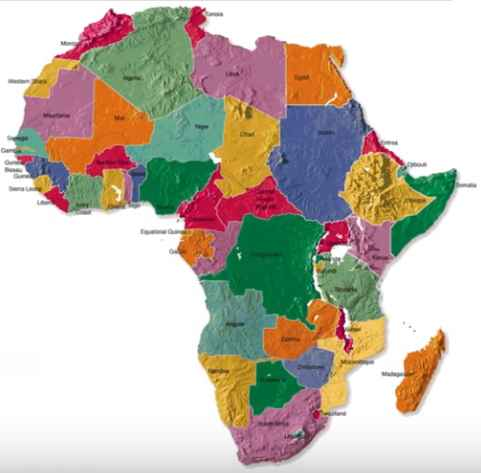
\includegraphics[width=0.8\textwidth]{MapColouring}
	\end{center}
\end{figure}

We know that 4 colours are enough: it turns out that the 3-Colour problem is \gls{gls:NP:complete}--Figure \ref{fig:naesat3colour}.
\begin{figure}[H]
	\caption[NAESAT $\le$ Graph 3-Colour]{NAESAT $\le$ Graph 3-Colour: each node is a country, and each border an edge; two nodes are connected \emph{iff} the two countries share a border.}\label{fig:naesat3colour}
	\begin{subfigure}[t]{0.45\textwidth}
		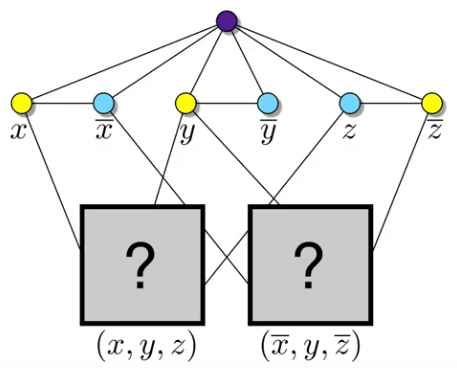
\includegraphics[width=0.8\textwidth]{naesat3colour}
	\end{subfigure}
	\begin{subfigure}[t]{0.45\textwidth}
		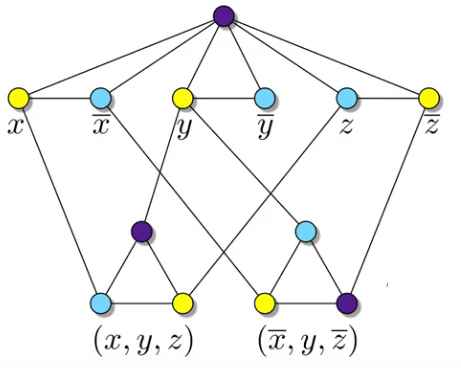
\includegraphics[width=0.8\textwidth]{naesat3solution}
	\end{subfigure}
\end{figure}

\begin{thm}[NAESAT $\le$ Graph 3-Colour]
	NAESAT $\le$ Graph 3-Colour
\end{thm}

\begin{proof}
	\begin{enumerate}
		\item Use gadgets to encode variables and enforce constraints.
		\item If there are two ways to colour something we call the colours ''true'' and ''false''--e.g. the triangles at the top.
		\item Assign an arbitrary colour to the topmost node.
		\item TBP
	\end{enumerate}
\end{proof}

3 colouring can be a disguise for any search problem--Hamiltonian path, TSP,...

\subsection{P versus NP Problem}

If any NP problem can be solved in polynomial time, then they all can, and $P=NP$. This would mean that any problem that is easy to check would also be easy to solve.

The question is still open, because we don't know all the possible ways to solve problems in polynomial time.

P and NP is about the nature of mathematical truth and creativity.

\subsection{Existence and Nonexistence }

A yes/no question is in NP if, whenever the answer is "yes", there is an easily checked proof or "witness" to that fact. Note there is an asymmetry, as we don't have to worry about "No". 

\subsection{Above and Beyond}

The class NP is about the existence of things: if it exists, and it is easy to check if you show it to me, then its in NP. As we go to deeper and more tangled relationships we find ourselves climbing through an infinite hierarchy--Figure \ref{fig:complexity:hierarchy}.

\begin{figure}[H]
	\caption{Complexity Hierarchy}\label{fig:complexity:hierarchy}
	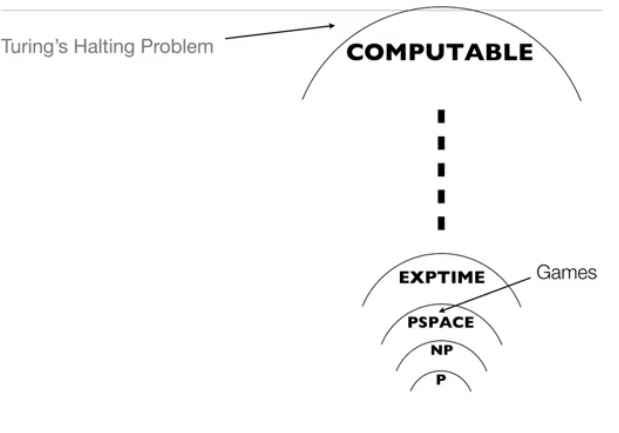
\includegraphics[width=0.8\textwidth]{hierarchy}
\end{figure}

Strategies are larger than Hamiltonian Paths: to prove that one side has a winning strategy I need to check an exponential path--Figure \ref{fig:PSPACE}. Playing games perfectly lives higher up in the complexity hierarchy--Figure \ref{fig:complexity:hierarchy}. 
\begin{figure}[H]
	\begin{center}
		\caption{Strategies are larger than Hamiltonian Paths}\label{fig:PSPACE}
		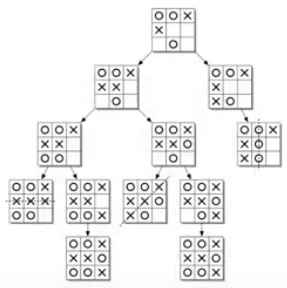
\includegraphics[width=0.6\textwidth]{PSPACE}
	\end{center}
\end{figure}

Exploring the tree could take exponential time, but, if the length of the game is polynomial, we only need polynomial space. We have another complexity class: \gls{gls:PSPACE}--\glsdesc{gls:PSPACE}

\begin{thm}
	$P \subseteq NP \subseteq PSPACE$
\end{thm}

\begin{proof}
	TBP
\end{proof}

We have a language to draw qualitative distinctions between problems, to locate them in the hierarchy of--Figure \ref{fig:complexity:hierarchy}.
\begin{quotation}
	Computers play the same role in complexity that clocks, trains, and elevators play on relativity--Scott Aaronson.
\end{quotation}

Computer science is not the study of computers, it is the study of computation.

\begin{figure}[H]
	\begin{center}
		\caption[Rule 110 is universal]{Rule 110 is universal\cite{cook2004universality}}
		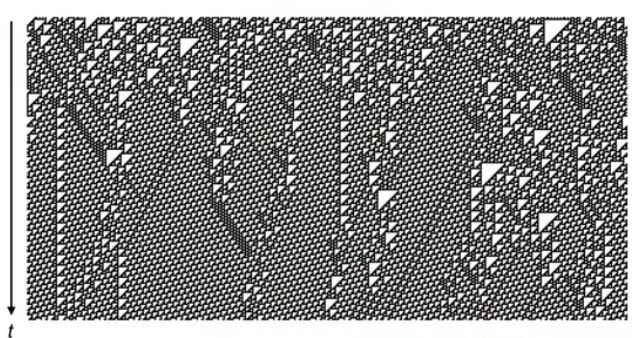
\includegraphics[width=0.8\textwidth]{rule110}
	\end{center}
\end{figure}

Given a cellular automaton, what questions can we ask about it?

\begin{enumerate}
	\item What will the state be at $t_{n+x}$?

	\item Does s have a predecessor?

	\item On a lattice of size $n$, is $s$ on a periodic orbit?

	\item On a lattice of infinite size, will $s$ ever die out?
	
\end{enumerate}

These all live at different levels of Figure \ref{fig:complexity:hierarchy}.

References: \cite[Chapters 4-6]{moore2011nature}, \cite{sep-computability}
\section{Worst-case, Natural, and Random}


\subsection{Real World Problems}

There are some gaps or bridges to cross between this theory and real world problems. \gls{gls:NP:complete}ness is a worst-case notion. Computer science assumes that instances are designed by a clever adversary to encode hard problems. For example, we showed that we could design a particularly hard graph colouring problem; this is good in cryptography, but not necessary in science. The solution to many physics problems are the simplest, most optimistic equation.

\begin{quote}
	The scientist is always working to discover the order and organization of the universe, and is thus playing a game against the arch enemy, disorganization. Is this devil Manichaean or Augustininan? Is it a contrary force opposed to order or is it the very absence of order itself?--Norbert Wiener, Cybernetics.
\end{quote}

Many algorithms that take exponential time in the worst case are efficient in practice.
Linear programming problems are a large class of optimization problems that include max flow and min cut. Solving them is like climbing to the top of a high dimensional jewel. There is an old algorithm, the simplex method, which is a simple greedy algorithm. People have dreamed up problems where the simplex method is exponential, but, in practice, real problems are typically tractable.

Spielman and Teng\cite{spielman2004smoothed} realized that noise foils the adversary, making a smoother problem: the number of facets goes down, and the path to the top get shorter. In the real world you never know the coefficients exactly, you never know exactly what the right hand side is. In the real world things are a wee bit noisy. Spielman and Teng observed that adding noise almost always makes the problem simpler. It greatly reduces the number of vertices on the path to the top, so the simplex algorithm will work efficiently (almost always).

\begin{figure}[H]
	\begin{center}
		\caption{Smoothed Analysis}\label{fig:hs-jewel}
		\begin{subfigure}[t]{0.45\textwidth}
			\caption{Optimization problems are like exploring a high dimensional jewel}
			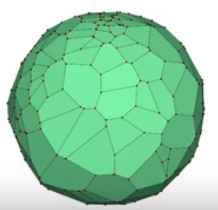
\includegraphics[width=\textwidth]{hs-jewel}
		\end{subfigure}
		\begin{subfigure}[t]{0.45\textwidth}
			\caption{Noise foils the adversary}
			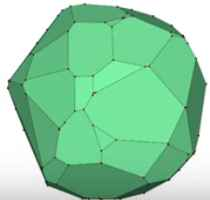
\includegraphics[width=\textwidth]{hd-jewel2}
		\end{subfigure}
	\end{center}
\end{figure}

There are hard examples of this problem, but they are rare and they are fragile. The adversary has to fine-tune the problem to make it hard. But there are other problems where we think hard problems are common and robust--e.g. cryptosystems.

Some real world problems are easy because of the structure of the landscape.

If you define clustering as optimization it is a hard problem, but it is one we solve every day. Why? Because of local minima. Maybe we are asking the wrong question: if there is one true clustering, it should be shouting at us, and there should not be other clustering that are almost as good but very different.

\begin{figure}[H]
	\begin{center}
		\caption[Some landscapes are not as bumpy as they could be]{Some landscapes are not as bumpy as they could be: if all good solutions are close to the optimum, cluster is easy. But if the landscape is really bumpy, maybe the pattern that we are looking for isn't really there.}\label{fig:rw-problems-easy}
		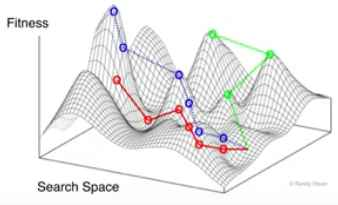
\includegraphics[width=0.6\textwidth]{rw-problems-easy}
	\end{center}
\end{figure}

Suppose the instance in front of you has the following structural property to its landscape of solutions:suppose that any local optimum that is almost as good as the global optimum is also close to the global optimum and agrees with it on most points. So there might be local foothills to the global optimum, but the global optimum dominates the landscape: you don't have another peak far away that is almost as high. Under this structural assumption Balcan, Blum and Gupta\cite{balcan2013clustering} showed that a certain clustering algorithm, similar to the k-means algorithm works very well and very quickly.

Another example of why real-world problems might be easy is protein folding. We have co-evolved the  sequences and the algorithms. If you look at energy, there is a nice deep bowl surrounding the correct conformation. Organism that live at higher temperatures have deeper bowls so the proteins won't accidentally get kicked out. 

So real world problems mostly have nicer landscapes than we'd expect from a diabolical adversary.
  
\subsection{Phase Transitions}

We have talked about the contrast between worst case problems that are designed by a nasty adversary and natural problems that we might encounter in the real world. It turns out that physics, especially statistical physics gives us a lot of machinery and mathematical techniques for thinking about the range of problems that we might encounter, and how the problems might get harder and their landscapes change as we increase the strength of their interactions and constraints. There are phase transitions between easy, hard, and insoluble.

We'll consider the Ising model.

\begin{figure}[H]
	\begin{center}
		\caption{Ising Model}
		\begin{subfigure}[t]{0.35\textwidth}
			\caption{: Atoms in a block of iron interact with their neighbours $\uparrow\uparrow\uparrow\downarrow\downarrow\uparrow\uparrow\downarrow\uparrow\uparrow\uparrow\uparrow$. When these interactions are strong enough and the temperature is low enough, the atoms line up and form a magnetic field.}
			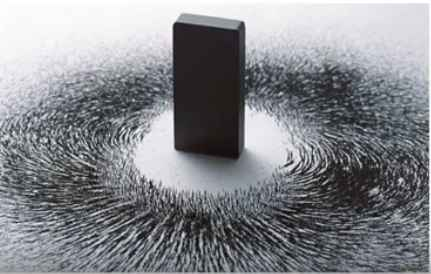
\includegraphics[width=\textwidth]{permanent-magnet}
		\end{subfigure}
		\;\;\;
		\begin{subfigure}[t]{0.6\textwidth}
			\caption{When iron is heated beyond the critical temperature, it suddenly loses its ability for hold a magnetic field. Below $T_c$ there is a clear majority of atoms favouring one direction, and they are organized into small islands; above $T_c$ the islands merge and the directions are random.}
			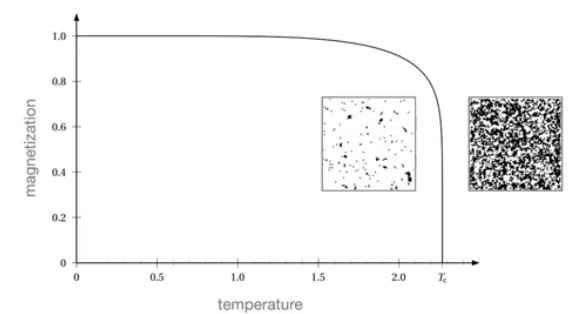
\includegraphics[width=\textwidth]{curie-temperature}
		\end{subfigure}
	\end{center}
\end{figure}


\subsection{Random Problems}

For NP problems, what happens when we pile up more and more constraints at random? At what point does it break so there is no longer a solution? We will focus on \gls{gls:3:SAT} with $n$ variables, $m$ clauses. For each clause choose a random triplet of variables and negate each with probability $\frac{1}{2}$. The interesting case is the sparse case $m=\alpha n$, for some constant density $\alpha$--analogous to spin glasses and random graphs. As we add constraints the probability of contradictions increases--Figure \ref{fig:trans}.

\begin{figure}[H]
	\caption[Transition from solvability to unsolvability]{Transition from solvability to unsolvability.}
	\begin{subfigure}[t]{0.45\textwidth}
		\caption{When the density of constraints is too high we can no longer satisfy them all at once.}\label{fig:trans}
		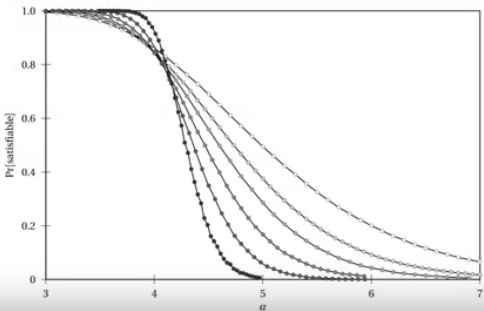
\includegraphics[width=\textwidth]{trans}
	\end{subfigure}
	\begin{subfigure}[t]{0.45\textwidth}
		\caption{Showing log of number of steps using the Davis Putnam search algorithm. Light grey dots correspond to satisfiable formulae, dark grey to unsatisfiable.\cite{davis1960computing}}\label{fig:dpll}
		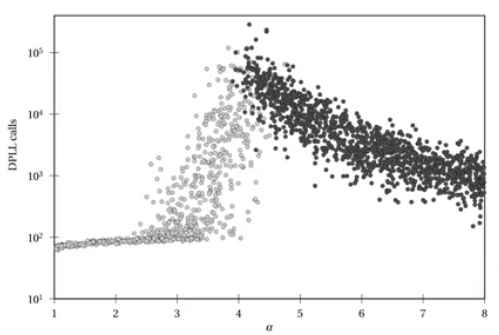
\includegraphics[width=\textwidth]{dpll}
	\end{subfigure}
\end{figure}

\begin{conj}[Threshold Conjecture]
	Let $F_k(n,m) = $ random \gls{gls:k:SAT} formula with n variables and m clauses. Then $\forall k \ge 3, \exists \alpha_k$ such that:
	\begin{align*}
		\lim_{n \rightarrow \infty} Pr\big[F_k(n,m=\alpha n)\big]\text{ is satisfiable}=&\begin{cases}
		1 \text{ if } \alpha<\alpha_k\\
		0  \text{ if } \alpha>\alpha_k
		\end{cases}
	\end{align*}
\end{conj}

If $k=2$ we can prove this from random graph theory.

In 2014 Jian Ding, Allan Sly, and Nike Sun proved that this is a theorem for $k$ sufficiently large\cite{ding2015proof}.

Fugure \ref{fig:dpll} depicts the difficulty of solving SAT problems as a function of $\alpha$. \begin{itemize}
	\item For small $\alpha$ it is easy, with hardly any backtracking.
	\item As $\alpha$ we have to work harder to find a solution.
	\item Maximum search time happens when we transition to unsolvability.
	\item As density continues to increase it gets easier to show that it is unsatisfiable. Contradicts arise and prune tree.
\end{itemize}

\subsection{Solvability Threshold}

\subsubsection{Bounding the threshold}
\begin{itemize}
	\item How many solutions does a random \gls{gls:3:SAT} formula have on average?
	\item There are $2^n$ vectors $X=(x_i)$. 
	\item Focus on one vector: for any particular random clause, the probability of it being satisfied is $\frac{2^3-1}{2^3} = \frac{7}{8}$.
	\item Since there are $m$ clauses, the probability of a random formula being satisfied is  $\big(\frac{7}{8}\big)^m$
	\item So the average number of solutions is $s^n\big(\frac{7}{8}\big)^m=\big[2\big(\frac{7}{8}\big)^\alpha\big]^n$
	\item This is exponentially small if $\alpha \ge \log_{\frac{7}{8}}2\approx5.15$
\end{itemize}

\begin{itemize}
	\item Let Z be the number of solutions.
	\item The average $E(Z)$ is exponentially small when  $\alpha \ge \log_{\frac{7}{8}}2\approx5.15$.
	\item Then Markov's inequality\cite{wiki:markov:inequality} tells us that $Pr\big(Z>0\big) \le E(Z)$ 
	\item So is $E(Z)$ is exponentially small, so is the probability of satisfiability.
	\item This proves that $\alpha_3<5.19$. But the true 3-SAT threshold is 4.27 (measured).
	\item In the gap $[4.27,5.19]$ we'd expect exponentially many solutions, but actually there aren't any! Why?
\end{itemize}

Figure \ref{fig:heavy-tail} depicts a Heavy Tail Distribution for Z: $E(Z)\ne$ typical value. This is the opposite of most classical statistics.
\begin{figure}[H]
	\begin{center}
		\caption{Heavy Tail Distribution: $E(Z)\ne$ typical value}\label{fig:heavy-tail}
		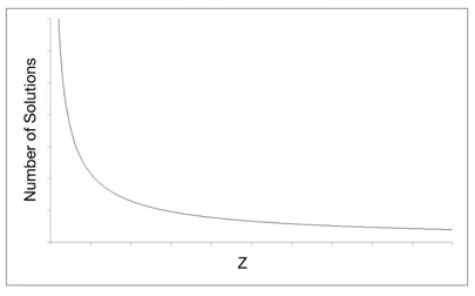
\includegraphics[width=0.6\textwidth]{heavy-tail}
	\end{center}
\end{figure}

Inequality is a one way street: $Pr\big(Z>0\big) \le E(Z)$, so if the expectation is small, so it the probability; but if the expectation is large, it does not imply that the probability is large. $E(Z)$ does not help us find a lower bound on the threshold.

Let us generalize from \gls{gls:3:SAT} to \gls{gls:k:SAT}, because it is interesting to ask how the threshold scales with $k$.

A random \gls{gls:k:SAT} clause is satisfied with probability $1-2^{-k}$. Following the same argument as before, $\alpha_k\le\frac{\log 2}{-\log (1-2^{-k})} \approx 2^k \ln(2)$. This is an upper bound, but it turns out to be pretty close: $\alpha_k=2^k \ln 2-O(1)$. Can we find solutions algorithmically all the way up to the threshold? Is there a zone where solutions exist but are hard to find?

\subsubsection{A simple search}

\begin{itemize}
	\item Setting a variable either satisfies a clause or shortens it.
	\item Setting $x$ false turns $(x\lor y \lor z)$ into $y \lor z$
	\item Setting $y$ false turns $(y \lor z)$ into $(z)$
	\item setting $z$ false turns $(z)$ into $()$--a contradiction.
\end{itemize}

A backtracking search would try another branch of the tree, but let's charge ahead and set variables permanently. We try another random branch instead. Maybe it will work if the density is low enough. We will try only one smart thing: if there is a unit clause, satisfy it. If there is no unit clause, choose a variable  with equal probability and give it a random value.

\subsection{Modelling Differential Equations}

\subsubsection{Modelling Differential Equations}
Following on from the algorithm at the end of the previous section, let's try to track the density of clauses of different lengths. We hope this very naive algorithm will find solutions for low enough density.

Since the formula is random, satisfying a unit clause has the same effect as giving a random variable a random value. It turns out that for random formulae we can analyze to process using differential equations.

We will track the number of clauses of different lengths: initially all clauses have the same length, but as we set variables clauses get shorter or disappear.

Imagine a variable in one clause being set to a value: either this clause demands that value, or some other clause does so. Probability that the variable gets the value that this clause demands in 0.5, so there are equal probabilities for eliminating or shortening clause. 

Let us say that there are $s_3n$ clauses of length 3, $s_2n$ of length 2, and we have set $tn$ variables so far. The expected values satisfy the following differential equations.

\begin{align*}
	\frac{d s_3}{dt} =& - \frac{3 s_3}{1-t}\\
	\frac{d s_2}{dt} =& \frac{\frac{3}{2}s_3-2s_2}{1-t}\\
	s_3(0)=& \alpha\\
	s_s(0)=& 0
\end{align*}

\begin{figure}[H]
	\begin{center}
		\caption{Solving the Differential Equations}
		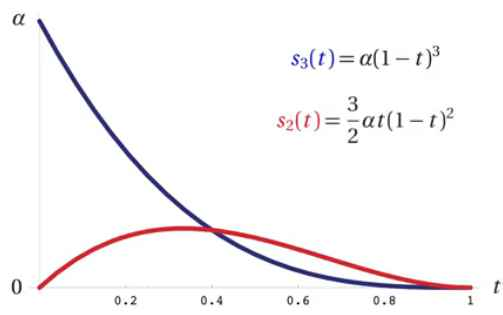
\includegraphics[width=0.8\textwidth]{solving-de}
	\end{center}
\end{figure}

From the Birthday Paradox, if we have $\sqrt{n}$ unit clauses it is likely that there is a contradiction. We don't want the number of unit clauses $\propto n$.

\subsubsection{Unit Clauses}

Unit clauses reproduce through the 1-variable clauses: $\bar{x}\land(x \lor y)\implies(y)$. We need the branching ratio (number of new clauses created when we satisfy one) or reproductive number.
\begin{align*}
	\lambda =& \frac{1}{2} \frac{2 s_2}{1-t}\\
	=& \frac{3}{2} \alpha t (1-t)
\end{align*}

\begin{itemize}
	\item If $\lambda>1$ the unit clauses reproduce faster than we can satisfy them.
	\item If $\lambda<1$ throughout, they stay under control and we can satisfy the entire formula. 
	\item $\lambda$ is maximized when $t=\frac{1}{2}$, $\lambda = \frac{3}{8} \alpha$
	\item $\alpha_3\ge\frac{8}{3}\approxeq2.667$ (Constructive proof)
	\item For \gls{gls:k:SAT} we can \emph{find} solutions up to a density of $\alpha = \Theta\big(\frac{2^k}{k}\big)$
	\item But we know there are solutions up to $\alpha_k=\Theta(2^k)$, some there is a gap between end of region where we can find solutions and where we know there are solutions--$\big[\frac{2^k}{k},2^k\big]$. Solutions exist, but maybe they are hard to find.
\end{itemize}

\subsection{Landscapes, Clustering, Freezing, and Hardness }

\subsubsection{Landscapes, Clustering, Freezing, and Hardness }

There is more to say about what's going on as we increase the density.
As you might imagine, the hardness of the problem has to do with the structure of the landscape. 
So remember how many optimization problems are hard once their landscapes, instead of having a single big peak, have lots of local optima.

Well, what happens in random SAT is very similar.
Imagine taking a topographic map of a mountain range and kind of slicing it off at a particular altitude, perhaps the altitude where indeed all of the clauses are satisfied.
If you have that Mount Fuji landscape, and you slice it off, then you get a nice big plateau of solutions.
And any solution in this rough area does pretty well and moreover, the set of solutions is connected to each other.
You could walk from any to any other by changing one variable at a time.
And there would be a way to do that while continuing to satisfy the entire formula.
Well, guess what?

As we increase the density, there is something called \gls{gls:clustering}--Figure \ref{fig:clustering-transition}. There are still many solutions but now, just as you get many mountain peaks in a hard problem, you now have little clusters of solutions, exponentially many clusters of solutions and not only are these separated from each other, but in order to get from one to the other, you would have to go down through a valley where you  dissatisfy a large number of clauses in order to travel from this cluster to that cluster.


\begin{figure}[H]
	\caption[Clustering, Freezing, and Hardness]{\gls{gls:clustering}: for $\alpha$ above this value, search algorithm gets stuck in whatever cluster it started in. \gls{gls:condensation}: a few clusters start to dominate. \gls{gls:freezing}: things get very brittle; in almost all clusters variables have to be set in a very specific way.}\label{fig:clustering-transition}
	\includegraphics[width=\textwidth]{clustering-transition}
\end{figure}



Physicists would say that this system has become glassy, and that you would have to cross over a difficult energy barrier to get from one cluster to another.
At that point, an algorithm which is trying to sample fairly, from all possible solutions, would have real trouble because, for instance, it was the kind of Monte Carlo algorithm, which is popular in many sciences, which runs around the space of possible solutions by flipping individual variables
Well it would be stuck in whatever cluster it started out in.
It would be very unwilling to pass through this zone of really bad nonsolutions in order to get to another cluster over there.
As we increase the density further, more structural transitions happen.
Again, these formulas are still satisfiable, but more things are happening to the set,
the structure, of solutions.

Above the clustering transition is another transition called the Condensation Transition--Figure \ref{fig:clustering-transition}.
At this point, a few of the clusters
dominate the set of possible solutions.
And if you're not lucky enough to start
out in one of them,
then in some sense you're not dealing
with a typical solution.

Beyond that is yet another transition, called the Freezing,
or Rigidity Transition--Figure \ref{fig:clustering-transition}.
Now, things are starting to get 
very brittle,
very tight.
Now, in almost all clusters,
most of the variables have to be set in
a specific way.
If they're not set in that way, there are
contradictions.
If you think about it, it is intuitive
that now a search algorithm
is in real trouble.

Let's say you start out kind of looking
down on this
vast space of possible solutions, if you
have no idea which way to go
you start setting variables and zooming
in on part of the solution space
hoping to find a viable cluster of
solutions there.
But, these clusters are frozen so that,
for instance, half their variables
have to be set precisely.
To particular values, or all solutions in
that vicinity will be disqualified.
Well, as you travel down your search tree
zooming in on parts of the space
you're setting more and more variables.
If you get even a single variable wrong,
setting it to the value that is opposite
to the one that's frozen into
that cluster then you're going to miss
that cluster completely.
You've gone down a branch of the
search tree below which there are no
solutions at all.
But you don't know that yet,
you're going to have to explore
that sub-tree and that will take you
exponential time.

So our current belief is that this 
Freezing Transition
is when this problem really gets hard.
That it really takes exponential time for
the types of algorithms that
anyone has been able to think of so far
to find even a single solution to the
random set problem.

So what's the lesson of all this?
It's not just this one transition at
the top
that takes us from satisfiable to
unsatisfiable,
there is a whole host of structural
changes that the landscape undergoes
some of which make it hard to sample
fairly
from the space of possible solutions
and some of it, some of which
we believe, make it hard even to
find a single solution
or tell if there is one.

\subsubsection{Solutions hidden behind energy barriers: glasses}

Imagine melting some silicon dioxide and cooling it down to make glass. At an atomic level the silicon dioxide is very amorphous--it looks more like a liquid than a crystal. The lowest possible energy is a perfect crystal, but they never get there. Little bits of crystal form in different places, but they conflict as they meet each other. As Figure \ref{fig:glass} depicts there is a very high energy barrier to the perfect configuration, and we are in a very high dimensional space, so it isn't clear what moved to make.

\begin{figure}[H]
	\begin{center}
		\caption[Solution hidden behind an energy barrier]{Solutions hidden behind an energy barrier with a narrow basin of attraction}\label{fig:glass}
		\includegraphics[width=0.8\textwidth]{glass}
	\end{center}
\end{figure}

The crystalline solution is an exponentially narrow fraction of all possible states. A glassy material can stay stuck in an amorphous state for exponential time, even though the minimum energy configuration is crystalline.

The same thing an happen to a search algorithm. It starts in a random state, and explores the space by flipping variables. There is a perfect solution in some tiny corner, but it will take exponential time to find it. The structure of these landscapes is what make these problems hard.

\subsubsection{XORSAT}

Returning to Figure \ref{fig:clustering-transition}:
\begin{itemize}
	\item all known algorithms for \gls{gls:k:SAT} atop working at $\alpha_{rigid}\approx \frac{2^k \log{k}}{k}$
	\item in between $\alpha_{rigid}$ and $\alpha_k=2^k \log(k)$, satisfiable but (we believe) exponentially hard.
\end{itemize}

Can this be made into a proof that $P\ne NP$? Actually, we don't \emph{know} that any of the above take exponential time, because we don't know whether $P$ and $NP$ are the same. People have tried to use the fitness landscape to prove that $P\ne NP$, but is doesn't really work. We can see this by introducing one more constraint satisfaction problem--\gls{gls:xorsat}.
\begin{align*}
	x_1 \oplus x_2 \oplus x_3 =& 1\\
	x_1 \oplus x_2 \oplus x_4 =& 0\\
	x_2 \oplus x_3 \oplus x_4 =& 1
\end{align*}

Random instances have many of the same problems as \gls{gls:3:SAT}: clustering, freezing, and a transition to unsatisfiability. But \gls{gls:xorsat} is easy: it is just a system of linear equations--because $\oplus$ is just a sum mod 2.
\begin{align*}
	\begin{pmatrix}
		1&1&1&0\\
		1&1&0&1\\
		0&1&1&1
	\end{pmatrix}\begin{pmatrix}
		x_1\\
		x_2\\
		x_3\\
		x_4
	\end{pmatrix}=&\begin{pmatrix}
		1\\
		0\\
		1
	\end{pmatrix}
\end{align*}

How is \gls{gls:xorsat} like \gls{gls:3:SAT}, and how is it different?
\begin{itemize}
	\item Clustering: local search algorithms can't explore the space, and global search algorithms get stuck in local optima.
	\item Freezing: backtracking algorithms take exponential time, repeatedly setting frozen variables the wrong way.
	\item 	But Gaussian elimination is a global change of variables, letting us turn a hard looking problem into an easy one.
	\item \gls{gls:xorsat} is in \gls{gls:P}!
	\item If SAT has a similar kind of rearrangement--something totally different from backtracking or local search $P=NP$!
	\item Proving that it doesn't is hard.
\end{itemize}

The landscapes for \gls{gls:xorsat} and \gls{gls:3:SAT} look similar, but solving linear equations involves a global rewrite of the system. The algoritms that fail for \gls{gls:3:SAT} fail for \gls{gls:xorsat} also.

References: \cite[Chapters 5,10]{moore2011nature}

\section{Computation Everywhere}

What is computation anyway? What are the basic building blocks you need to perform computation? What does a complex system need to possess in order to compute? What are the simplest object that suffices?
\subsection{Building Blocks: Recursive Functions}
We will start with David Hilbert's Entscheidungsproblem, 1928: is there an effective procedure which, given a set of axioms and a mathematical problem, can decide whether the proposition is provable from the axioms? Unfolding the definition of an  effective procedure was one of the major issues in 20th century mathematics.

What functions of the natural numbers are computable? Major players: Richard Dedekind, Thoralf Skolem, R\'osza P\'eter

Axioms: let is assume that $0(x)=0$, $(x)=x$, and $S(x)=x+1$ are computable. Then we form new computable functions recursively from the old ones. What rules should we allow?

\begin{itemize}
	\item Composition: if $f$ and $g$ are computable, $h(x) = f(g(x))$ is computable.
	\item Primitive recursion: if $f$ and $g$ are computable, then $h$ is computable, where:
	\begin{align*}
			h(x,0) =& f(x) \text{, base case}\\
			h(x,y+1) =& g(x,y,h(x,y))
	\end{align*}
\end{itemize}

\glsdesc{gls:pr} The \glspl{gls:pr} already include a large group of functions.

\subsection{Building Blocks: Partial Recursive Functions}

Do we really need while loops?

Minimization or $\mu$-recursion: $h(x)=$ the smallest $y$ such that $f(x,y)=0$. What if $f(x,y)>0 \; \forall y$? Then loop never returns--$h$ undefined. Partial function.

Are there total function (always defined) that are partial recursive but not primitive recursive? Consider the Ackermann function

\begin{align*}
	A(1,x,y) =& x+y\\
	A(2,x,y) =& x \cdot y\\
	A(3,x,y) = x^y\\
	A(4,x,y) = x^{x^x} \rbrace \text{ $y$ times}
\end{align*} 

$A(n,x,y)$ requires $n$ nested for loops, so we need \emph{while}.

\subsection{$\lambda$ Calculus}

A system based entirely on strings and substitution. $\lambda x$ means "replace every occurrence of $x$ with a copy of the following string". E.g.

\begin{align*}
	(\lambda x.xx)a=&aa\\
	(\lambda x.xx)(ab)=&(ab)(ab)
\end{align*}

We can form functions of several variable, e.g.
\begin{align*}
	(\lambda xy.xyx)(ab)(c) =& (\lambda y.(ab)y(ab))c \text{, substituting $x$}\\
	=& (ab)c(ab) \text{, on substituting $y$}
\end{align*}

In the $\lambda$ Calculus there is no distinction between functions and data. $\lambda fx.f(fx)$ takes a function $f(x)$ and returns $f(f(x))$.

In chemistry RNA and proteins can take each other as input, acting both as functions and data--Walter Fontana.

We need a way to encode the integers (Church numerals):
\begin{align*}
	0=&\lambda fx.x\\
	1=&\lambda fx.fx\\
	2=&\lambda fx.f(fx)\\
	3=&\lambda fx.f(f(fx))
\end{align*}

Sometimes substitution never ends:
\begin{align*}
	(\lambda x.xx)	(\lambda x.xx) =& (\lambda x.xx)	(\lambda x.xx)\\
	=&...
\end{align*}

\begin{itemize}
	\item Self reproduction, like a program printing its own source. 
	\item A program that never halts, or an undefined function.
	\item Can we tell whether a string will ever settle down?
\end{itemize}

\subsection{Turing Machines}

So we've talked about the
partial recursive functions,
we've talked about
the lambda calculus,
these were two of
the models of computation,
and definitions of
what is computable
that were proposed
in the first half
of the Twentieth Century.
And notice that they looked
totally different from each other,
they looked, like,
utterly, completely
different beasts.
But we found that there were ways
that the lambda calculus
could simulate
some arithmetic
and we even built the successor function
in the lambda calculus
which was one of
the basic building blocks
of the partial recursive functions.
So you may already
be getting the idea
that, although these different models
of computation are very different,
they can simulate each other
to some extent.

Well, in some sense
this debate about
what is computational,
what is computable,
it may not have ended,
but it reached a huge milestone
when we came to
the Turing machine.

\subsubsection{Turing Machines}

So, Turing machine was invented
by Alan Turing, who hopefully
you've heard of for lots of reasons,
including helping,
actually playing a leading role
in decoding the Nazi Enigma code,
coming up with mathematical models
of pattern formation in biology,
like embryogenesis, how
fly embryos get the segments
of their thorax,
or for that matter
how leopards get their spots,
and also being persecuted
by the government
for his homosexuality
and being driven to suicide by it,
which was an enormous loss
for the world, and especially for mathematics and computer science.

So, here is his definition of a basic computer--Figure \ref{fig:TuringMachine}:

\begin{enumerate}
	\item we have a tape and on this tape are written symbols in some finite alphabet. These could be zeroes and ones, they could be A through Z, just some finite set.

	\item Then we have a head which moves back and forth on the tape. The head is a very simple machine and it only has a finite set of states, which we'll call "S."
	
	\item Now, all this machine can do at each step is read the symbol, at its current location on the tape. 	It may then, depending on that symbol 	and its internal state, 	so depending on "a," the tape symbol 	and S, its internal state, 	it may do a very small handful of things.
	
\begin{itemize}
	\item 	It may 	write a new symbol 	at that location on the tape,
	overwriting the "a" with something new, $a^\prime$,
	\item and it may then move 	left or right by one step.
\end{itemize}
	And that's all it does.
\end{enumerate}


\begin{figure}[H]
	\begin{center}
		\caption{A Turing Machine}\label{fig:TuringMachine}
		\includegraphics[width=0.8\textwidth]{TuringMachine}
	\end{center}
\end{figure}

So any Turing machine
can be described
just in terms of
the alphabet of tape symbols "a,"
the set of finite states S
for the head,
and what we call the
transition function,
$F: A \times S \rightarrow A \times S \times \{Left,Right\}$.

You can think of this almost as a simple electric device which is moving back and forth
on some magnetic tape or something. It looks like something that you could really build.

We're going to add one more thing, there's going to be a special state which we'll call "halt" when the machine is done. So how would it actually carry out a computation?
We would give it its input by writing some initial string; it could be a string of bits
representing an integer, it could be a string of letters or whatever, on its tape.

We then set it up in a special initialized state--I guess that's another special state--
and we let it go and it does whatever it's going to do, reading and writing, shuttling back and forth, until it reaches the halt state, and then its output is what is then written on the tape.



\subsubsection{Universal Turing Machines}

So, Turing machines, we just saw, can compute the successor function.
It's intuitively clear that they can also carry out composition.
If I have a Turing machine which computes
one function, $f$, and then halts, and another Turing machine which computes another function, $g$, and then halts, well I can compose these two functions by running one of these Turing machines and then running the other one.
And what I really mean is I would build a third Turing machine
where it has the combination of the two Turing machines state spaces and, when the first one halts and completes its work, that makes the transition to the initial state
of the second Turing machine, which then goes to work until it halts.

In fact, it might not surprise you
that Turing machines can do
all of the things
that partial recursive functions can do.
So, but,
Turing also found something quite lovely
and he actually designed one,
there are universal Turing machines
that can simulate any other
Turing machine.
How do we do that?
Well, you know, just as a program is,
can be viewed
simply as a text file
that you would hand as input
to another program,
I just told you that Turing machines
can be described completely
in terms of their transition functions.
So I could put
the description of one Turing machine
on the tape
of another Turing machine,
along with an input,
and then I could set this
universal Turing machine loose,
and it could, in theory,
simulate this Turing machine
on that input
and produce the results.
And, in fact,
there are Turing machines
which do exactly this.
We could call them <i>U</i>,

And what <i>U</i> does
is it takes a pair of things as input,
<i>P</i>, which you can think of
as a program
or the description for
another Turing machine,
and the input <i>x</i>
and <i>U</i> given the pair,
<i>P comma x</i>
produces
<i>P of x</i>:
what <i>P</i> would do
given input <i>x</i>.
$U(P,x)=P(X)$
Now, in the modern age,
this doesn't sound particularly
interesting or surprising,
because what is an operating system?
An operating system is a program
which runs programs.
So right now on your laptop
or your phone
or what have you,
is a program running all the time
which, when you give it a program,
it says, okay, I'll run this program
for you.
It's a program which runs programs.

An interpreter
is a program
which takes another program as input
and goes through it step by step
and simulates it.
And indeed,
people write interpreters
in undergraduate programming courses.
But in 1936,
when Turing was coming up with this,
this was a big, profound fact.
Again, think about
classical mathematics.
Can you think of a function
which you can give as its input
a description of other functions
and it will carry out any function
you give it?
That sounds absurd.
In order to carry out a function,
you need some higher order thing,
like a mathematician,
or a calculator.
Functions don't carry out
other functions.
And there's certainly no
universal function
which can carry out
any function at all.

And yet,
in the world of Turing machines,
you have exactly that.
Turing's original universal machine
was quite large,
with a lot of symbols,
and a lot of states.
But in fact clever people
have come up with very small
universal Turing machines,
with as few as four tape symbols
and six states,
for instance.
So, this phenomenon of
universal computation
is pretty ubiquitous,
you don't even need
that big a machine
to be capable of universality.

\subsection{The Halting Problem}

Is there a computer program that predicts (in finite time) whether any other program eventually halts? This would help answer unsolved mathematical problems such as Goldbach's conjecture: just write a program to find a counterexample, then check whether it halts--Figure \ref{fig:midgard-serpent}

\begin{figure}[H]
	\begin{center}
		\caption{The Midgard Serpent}\label{fig:midgard-serpent}
		\includegraphics[width=0.8\textwidth]{midgard-serpent}
	\end{center}
\end{figure}
Is there a program (a computable function) $Halts(P,x)$ that predicts, in finite time, whether program $P$ halts given input $x$? If there were, we could ask it about itself--Algorithm \ref{alg:mobius}.

\begin{algorithm}[H]
	\caption{M\"obius}
	\KwData{P}
	\KwResult{whether P halts }
	 \eIf {Halts(P,P)} {run forever:}
	 {Halt}\label{alg:mobius}
\end{algorithm} 

Does M\"obius(M\"obius) halt or not?
\begin{itemize}
	\item if it halts it runs forever;
	\item if ir runs forever it halts!
\end{itemize}

The only way out of this contradiction is if halts is undecidable: $Halts$ does not exist! There is a question about computer programs which no well-defined program can answer.

\begin{thm}[Rice]
	Any question about the long term behaviour of a Turing Machine is undecidable, since we can reduce the Halting problem to it.
\end{thm}

\subsection{The Grand Unified Theory of Computation}

\subsection{The Analytical Engine}

\subsection{Cellular Automata}
So,
Babbage's machine,
if he could have built it,
would have been able
to carry out
any computation that modern computers can
although it would have needed
a lot of space and a lot of steam.
What else is capable
of universal computation?

Well, in complex systems
we kind of enjoy
and love
these little examples,
these toy universes,
cellular automata.
So, a cellular automaton is something
typically a 1- or 2-dimensional grid
and at each grid location
we have a finite set of states,
and one of our favorite examples
also a popular screensaver
is The Game of Life
invented by John Conway.

So in The Game of Life,
each grid square can be alive or dead.
Here the alive things are black
and the dead things are white.
And, as in all cellular automata,
there is a simple, local rule
where each grid point,
at each step, looks at
its own state and those of its neighbors
and then computes its new state
and everything gets updated in parallel.

In this particular rule,
the neighbors are the 8 locations
in the grid that you could move to
with the move of a chess king
and the rule goes like this:
if you are alive,
and 2 or 3 of your 8 neighbors are alive,
you stay alive.
If fewer than 2 are alive,
you die of loneliness.
If 4 or more are alive,
you die of overpopulation,
goes the story.
This isn't really a biological model,
but. Okay, and
if you are dead, your square is empty,
and you have exactly 3 neighbors
that are alive,
then on the next step
you will be alive.
That's the whole rule.
And Conway played with these
numbers, these thresholds, for
being alive or dead until
it did something fun and interesting,
basically.

So one of the things that happens
in The Game of Life is
a little thing we call a "glider."
It's this little wiggly animal
which travels across diagonally,
and it will keep traveling until it
bumps into something.
Then, there's another thing
called a "glider gun,"
which shuffles back and forth,
and produces a stream of gliders.
And moreover it's possible
to carefully design collisons
between the gliders,
to build small objects,
or even to carry out logical operations.
We can use the gliders,
a stream of gliders,
almost like a wire,
to carry a bit of information.
Well, if you combine
all of these elements,
and you're extremely clever
and you have an abundance of free time,
you can build a Turing machine
out of The Game of Life.

So here we have
a very complicated configuration
in which the pixels are
almost too small to see.
I've zoomed in on
one of the glider guns there,
where, across the diagonal here
we have the Turing machine's tape,
and here we have the head
of the Turing machine.

And so The Game of Life
with a large enough initial configuration,
can simulate a Turing machine.
There are some interesting questions
here about is it okay
to start with a configuration
which is infinite, but periodic.
That gives you all the tape
you could ever possibly need,
or, perhaps there's a clever way
to have glider guns build the tape
over time, starting with
an initial configuration which is blank,
outside of a finite area.

But, anyway.
The Game of Life can compute.
It can compute because I just showed you
how to build a computer in it.
Remember a long time ago
when we were talking about
the NP-Completeness of certain problems
like, ah, like the tiling problem,
fitting in puzzle tiles
into a certain shape,
or the Hamiltonian path problem,
and I emphasized
that these problems are hard because
you can build computers out of them.

Well, here we're building
universal computers,
and given enough space and time,
in a cellular automaton,
we can carry out
<i>any</i> computation at all,
not just one in say,
polynomial time or exponential time,
the way we were talking about before.
The Game of Life is a 2-dimensional
cellular automaton,
in which it's fairly easy
to set up a tape,
and a head which moves back and forth
on that tape.
So what about 1-dimensional
cellular automata?
Well, here is a particular
1-dimensional cellular automaton.
Again, we just have 2 states,
0 and 1, or black and white,
at each location,
and, again,
we look at our nearest neighbors
as well as our own state,
and this is the update rule
where I'm showing you
what the new state will be
for the 8 possible neighborhoods,
combinations of your own state
and those of your neighbors.
In fact, this is cellular automaton
Rule 110
because, if these black squares are ones
in the rule
and the white squares are zeroes,
then in binary,
this spells out 110.

And Stephen Wolfram invented
that numbering scheme
as a way of exploring
all cellular automaton rules
of a given size.
So, here is a space-time diagram
of a typical run of Rule 110.

At the top we have

the top row is some initial

setting, of all the cells in the grid,

and time goes downward.

And when you look at this,

what immediately jumps out at you

is there are all kinds of gliders.

There are all sorts of different

particles, if you will, analogous to

the glider in The Game of Life,

but with many types,

which, as we move down,

may move left or right

at various velocities,

and you can see that

when they bump into each other,

complicated things happen.

So, it's tempting to think

that we can build a Turing machine

out of this.

This was conjectured by Stephen Wolfram

and then proved by Matthew Cook,

and the two of them published this paper

and showed that indeed, Rule 110

is capable of universal computation

and, therefore,

its long-term behavior,

what will eventually happen

from some initial state,

is undecidable.

And Turlough Neary and Damien Woods

improved their simulation,

and showed that, in fact, it can simulate

Turing machines with only

polynomial overhead; in other words,

it can simulate t steps

of a Turing machine

with an amount of time

which is only polynomial NT.

That means that predicting it,

even for finite time,

requires you to do a fair amount of work,

about as much work as you

would need to run a Turing machine

for that amount of time.

\subsection{Tile-Based Computation}

In, in this one-dimensional Turing machine

each row is another time step,

and so the space-time diagram

is two-dimensional.

We have one space dimension

and one time dimension.

So, what about another question

in two dimensions,

which is analagous

to our NP-Complete question

that we had of whether

tiles of a certain shape

can be placed

to fill in with no gaps or overlaps

a certain target overall shape.

But let's ask an infinite version

of this question.

So, Wang tiles

are little squares

where on each of their edges

there is a color,

and, when we stick them together,

these colors have to match

along their shared edge.

So, there's a nice question here,

if I give you

a finite set of these Wang tiles,

I can ask you,

can you cover the entire

two-dimensional plane with them--

an infinite configuration

where every place where two tiles meet,

their colors match.

In this particular example,

we can cover this 3x3 square

and then we notice something nice:

the colors along the top row

match those along the bottom row,

and the colors along the left edge

match those along the right edge,

which means that we can repeat

this configuration infinitely

and cover the entire plane

with this periodic configuration.

All right.

But, when can you do this

and when can't you?

Well, guess what?

Wang tiles can simulate a Turing machine.

Here's a little sketch of how to do this.

Some of our tiles represent

tape symbols,

and they're colored in such a ways

that we go from one row to the next,

they simply repeat that tape symbol,

carrying it across to the next step

of the computation.

Some other tiles

represent a combination

of a tape symbol and a head,

the head of the Turing machine,

which is in a particular state.

And, we again arrange the colors

so that the only way to continue

the tiling from one row to the next

is to carry out one step

of the Turing machine,

both updating the tape symbol

and updating the state.

So, this means

that asking whether I can tile

the entire plane,

corresponds to the halting problem

because if each row is a new step

of the Turing machine,

suppose I arrange things so that

the halting state

is some kind of gap

with no allowed tile

that I can fit in there.

Well, then, the question of whether

I can continue the tiling forever

and cover the entire plane

is exactly the question of whether

the Turing machine will run forever

and never halt.

Now, there is a catch,

which you may have already noticed.

If you hand me this bunch of tiles,

and ask me whether I can tile the plane,

why can't I cheat,

and just avoid the head of the

Turing machine completely,

and cover the entire plane

with just an empty tape,

which is repeating the same symbol

over and over,

with no Turing machine in sight

reading or writing anything

or with any danger of halting.

Well, this is a good point,

and, in fact, when the Wang tiles

were first invented, it was conjectured

that any set of tiles

that could tile the plane at all,

could do so periodically.

And if you think about it,

if that were so,

then the tiling problem would be

decidable.

Because we would just look at

larger and larger areas,

and we would eventually

either find an area which we could tile

in a way that we can repeat everywhere,

because the colors match along,

just as before,

match along the top and bottom edges

and the left and right edges,

or,

we would reach a finite area

which can't be tiled at all,

and one way or the other

we would know.

But that conjecture was wrong.

There are <i>aperiodic</i> tilings.

There are sets of tiles that can cover

the entire plane,

but only do so

in a funky way

which never quite repeats.

So here is a picture

of the classic Penrose tiles,

with these kites and darts

which, because of their local

5-way symmetry

have to tile the plane aperiodically,

because there's no periodic tiling

with perfect 5-way symmetry.

Now, I wanted to show you these

because they're beautiful,

but,

the Wang tiles is really more of

a question about square grid,

so, can we do something similar,

with tiles that line up with each other

on a square grid,

but somehow because of their colors,

or their shapes,

or maybe little doodads we add to them,

they <i>only</i> tile the grid

in an aperiodic way.

Well indeed this is possible,

and this is a particular setup

discovered by the logician

Raphael Robinson.

These tiles can only cover the grid

in a particular fractal pattern,

and so with this fractal pattern

we can with a little work

force

the Turing machine we're simulating

to first of all, exist

by demanding that there is a head

there at the upper left-hand corner,

and we can force it to attempt

longer and longer computations

until if at some point it halts,

there will be a place in the tiling

that we cannot fill in.

\subsection{Dynamical Systems} 

\subsubsection{Dynamical Systems} 

\subsubsection{Baker's Map}

References: \cite[Chapter 7]{moore2011nature}.

% end of text 

% glossary

\printglossaries

% bibliography go here
 
\bibliographystyle{unsrt}
\raggedright
\addcontentsline{toc}{section}{Bibliography}
\bibliography{computations}

\end{document}
